\hypertarget{md5_8h}{
\section{md5/md5.h File Reference}
\label{md5_8h}\index{md5/md5.h@{md5/md5.h}}
}
Diese Funktionen liefern die Moeglichkeit, einen MD5-Hash eines beliebigen String zu generieren. 



This graph shows which files directly or indirectly include this file:\nopagebreak
\begin{figure}[H]
\begin{center}
\leavevmode
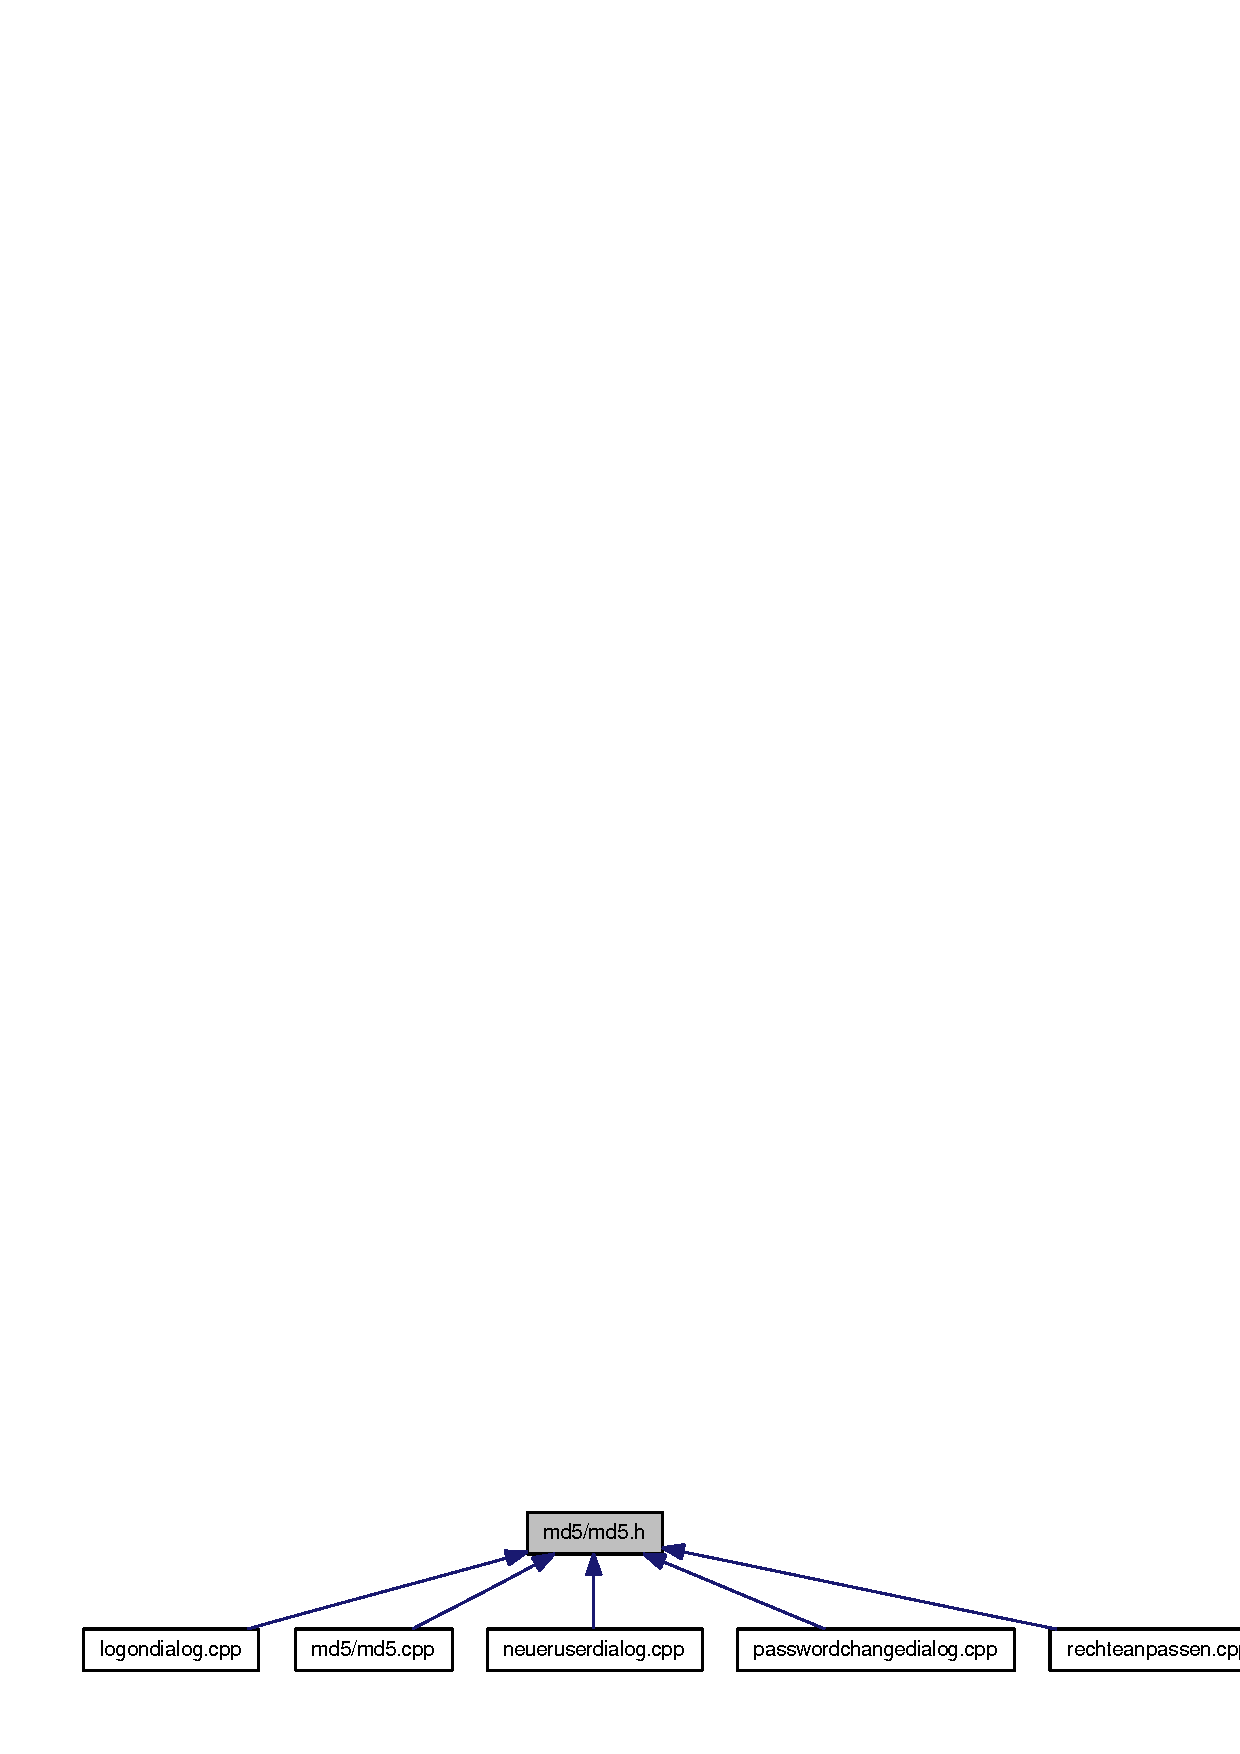
\includegraphics[width=306pt]{md5_8h__dep__incl}
\end{center}
\end{figure}
\subsection*{Classes}
\begin{CompactItemize}
\item 
struct \hyperlink{structmd5__t}{md5\_\-t}
\end{CompactItemize}
\subsection*{Defines}
\begin{CompactItemize}
\item 
\#define \hyperlink{md5_8h_346b45663bfa5a41fb49acad0845bfd8}{MD5\_\-SIZE}~16
\item 
\#define \hyperlink{md5_8h_115bf68d9f4ca75cd56221a136ce689c}{MAX\_\-MD5\_\-UINT32}~((\hyperlink{md5_8h_a5370400843756f0b77b782bdeef2564}{md5\_\-uint32})4294967295U)
\item 
\#define \hyperlink{md5_8h_8306a54d7d4073b1efe9602be8b1ba8d}{MD5\_\-BLOCK\_\-SIZE}~64
\end{CompactItemize}
\subsection*{Typedefs}
\begin{CompactItemize}
\item 
typedef unsigned int \hyperlink{md5_8h_a5370400843756f0b77b782bdeef2564}{md5\_\-uint32}
\end{CompactItemize}
\subsection*{Functions}
\begin{CompactItemize}
\item 
void \hyperlink{md5_8h_eb46e2a63662d4994071a043b5f7f6c7}{md5\_\-init} (\hyperlink{structmd5__t}{md5\_\-t} $\ast$md5\_\-p)
\item 
void \hyperlink{md5_8h_4560b471c3530ca3b13a8c9cfcb59761}{md5\_\-process} (\hyperlink{structmd5__t}{md5\_\-t} $\ast$md5\_\-p, const void $\ast$buffer, const unsigned int buf\_\-len)
\item 
void \hyperlink{md5_8h_72e5f2ef4e06c2db4f98b15a2de5228b}{md5\_\-finish} (\hyperlink{structmd5__t}{md5\_\-t} $\ast$md5\_\-p, void $\ast$signature)
\item 
void \hyperlink{md5_8h_975b91095e7b86642f360d060dd2f8db}{md5\_\-buffer} (const char $\ast$buffer, const unsigned int buf\_\-len, void $\ast$signature)
\item 
void \hyperlink{md5_8h_0f4331b29464a71b266fda74c0edd8a7}{md5\_\-sig\_\-to\_\-string} (void $\ast$signature, char $\ast$str, const int str\_\-len)
\item 
void \hyperlink{md5_8h_47c9c3ea0284cf6283dc3de13a181c0a}{md5\_\-sig\_\-from\_\-string} (void $\ast$signature, const char $\ast$str)
\end{CompactItemize}


\subsection{Detailed Description}
Diese Funktionen liefern die Moeglichkeit, einen MD5-Hash eines beliebigen String zu generieren. 

\begin{Desc}
\item[Version:]1.7 \end{Desc}
\begin{Desc}
\item[Date:]05.03.2006 \end{Desc}
\begin{Desc}
\item[Author:]Gray Watson \end{Desc}


Definition in file \hyperlink{md5_8h-source}{md5.h}.

\subsection{Define Documentation}
\hypertarget{md5_8h_115bf68d9f4ca75cd56221a136ce689c}{
\index{md5.h@{md5.h}!MAX\_\-MD5\_\-UINT32@{MAX\_\-MD5\_\-UINT32}}
\index{MAX\_\-MD5\_\-UINT32@{MAX\_\-MD5\_\-UINT32}!md5.h@{md5.h}}
\subsubsection[MAX\_\-MD5\_\-UINT32]{\setlength{\rightskip}{0pt plus 5cm}\#define MAX\_\-MD5\_\-UINT32~(({\bf md5\_\-uint32})4294967295U)}}
\label{md5_8h_115bf68d9f4ca75cd56221a136ce689c}




Definition at line 62 of file md5.h.

Referenced by md5\_\-finish().\hypertarget{md5_8h_8306a54d7d4073b1efe9602be8b1ba8d}{
\index{md5.h@{md5.h}!MD5\_\-BLOCK\_\-SIZE@{MD5\_\-BLOCK\_\-SIZE}}
\index{MD5\_\-BLOCK\_\-SIZE@{MD5\_\-BLOCK\_\-SIZE}!md5.h@{md5.h}}
\subsubsection[MD5\_\-BLOCK\_\-SIZE]{\setlength{\rightskip}{0pt plus 5cm}\#define MD5\_\-BLOCK\_\-SIZE~64}}
\label{md5_8h_8306a54d7d4073b1efe9602be8b1ba8d}


The MD5 algorithm works on blocks of characters of 64 bytes. This is an internal value only and is not necessary for external use. 

Definition at line 68 of file md5.h.

Referenced by md5\_\-finish(), and md5\_\-process().\hypertarget{md5_8h_346b45663bfa5a41fb49acad0845bfd8}{
\index{md5.h@{md5.h}!MD5\_\-SIZE@{MD5\_\-SIZE}}
\index{MD5\_\-SIZE@{MD5\_\-SIZE}!md5.h@{md5.h}}
\subsubsection[MD5\_\-SIZE]{\setlength{\rightskip}{0pt plus 5cm}\#define MD5\_\-SIZE~16}}
\label{md5_8h_346b45663bfa5a41fb49acad0845bfd8}


Size of a standard MD5 signature in bytes. This definition is for external programs only. The MD5 routines themselves reference the signature as 4 unsigned 32-bit integers. 

Definition at line 55 of file md5.h.

Referenced by md5\_\-sig\_\-from\_\-string(), and md5\_\-sig\_\-to\_\-string().

\subsection{Typedef Documentation}
\hypertarget{md5_8h_a5370400843756f0b77b782bdeef2564}{
\index{md5.h@{md5.h}!md5\_\-uint32@{md5\_\-uint32}}
\index{md5\_\-uint32@{md5\_\-uint32}!md5.h@{md5.h}}
\subsubsection[md5\_\-uint32]{\setlength{\rightskip}{0pt plus 5cm}typedef unsigned int {\bf md5\_\-uint32}}}
\label{md5_8h_a5370400843756f0b77b782bdeef2564}


NOTE: the following is assumed to generate a 32-bit unsigned data type. 

Definition at line 61 of file md5.h.

\subsection{Function Documentation}
\hypertarget{md5_8h_975b91095e7b86642f360d060dd2f8db}{
\index{md5.h@{md5.h}!md5\_\-buffer@{md5\_\-buffer}}
\index{md5\_\-buffer@{md5\_\-buffer}!md5.h@{md5.h}}
\subsubsection[md5\_\-buffer]{\setlength{\rightskip}{0pt plus 5cm}void md5\_\-buffer (const char $\ast$ {\em buffer}, \/  const unsigned int {\em buf\_\-len}, \/  void $\ast$ {\em signature})}}
\label{md5_8h_975b91095e7b86642f360d060dd2f8db}


DESCRIPTION:

This function is used to calculate a MD5 signature for a buffer of bytes. If you only have part of a buffer that you want to process then md5\_\-init, md5\_\-process, and md5\_\-finish should be used.

\begin{Desc}
\item[Returns:]None.\end{Desc}
\begin{Desc}
\item[Parameters:]
\begin{description}
\item[{\em buffer}]A buffer of bytes whose MD5 signature we are calculating.\item[{\em buf\_\-len}]The length of the buffer.\item[{\em signature}]A 16 byte buffer that will contain the MD5 signature. \end{description}
\end{Desc}


Definition at line 483 of file md5.cpp.

References md5\_\-finish(), md5\_\-init(), and md5\_\-process().

Referenced by LogonDialog::on\_\-LogonButton\_\-released(), RechteAnpassen::on\_\-okButton\_\-released(), PasswordChangeDialog::on\_\-okButton\_\-released(), and NeuerUserDialog::on\_\-okButton\_\-released().

Here is the call graph for this function:\nopagebreak
\begin{figure}[H]
\begin{center}
\leavevmode
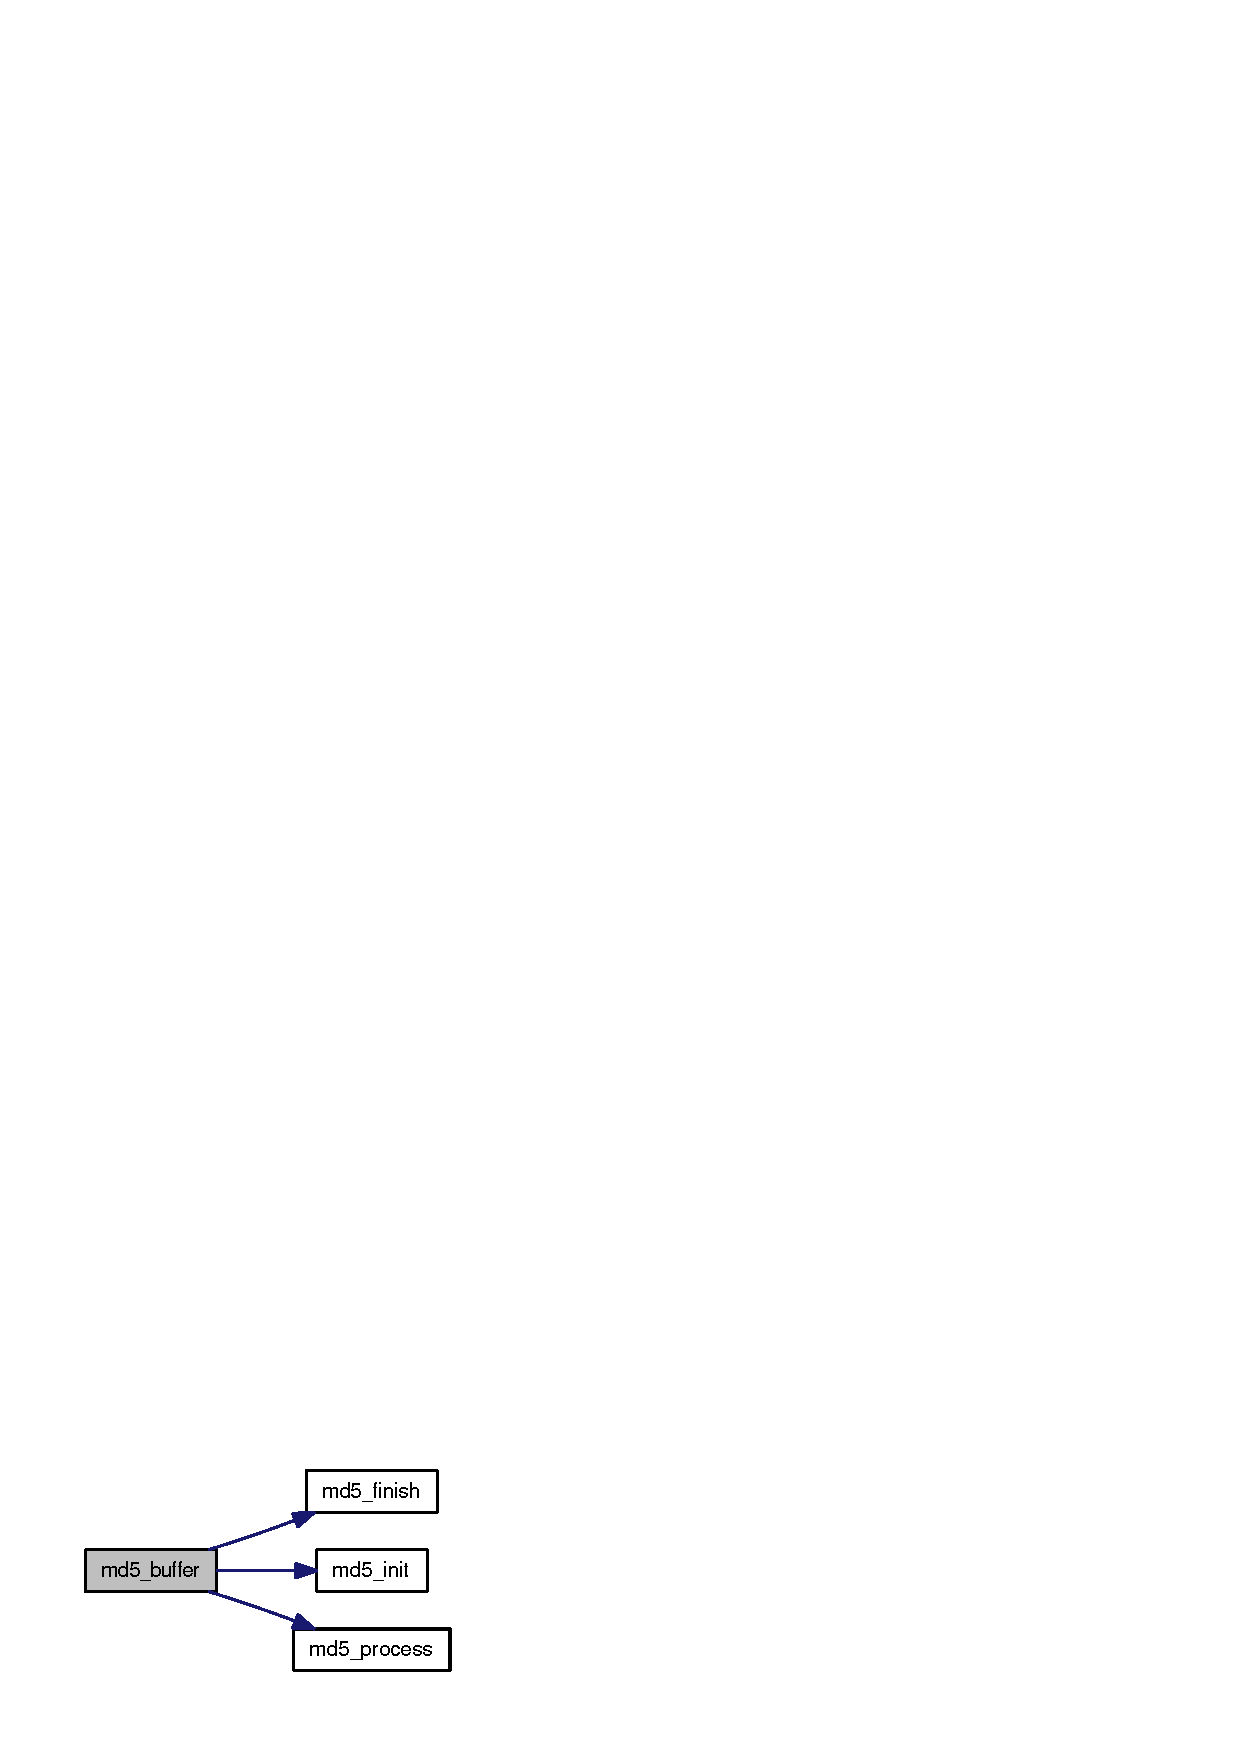
\includegraphics[width=110pt]{md5_8h_975b91095e7b86642f360d060dd2f8db_cgraph}
\end{center}
\end{figure}
\hypertarget{md5_8h_72e5f2ef4e06c2db4f98b15a2de5228b}{
\index{md5.h@{md5.h}!md5\_\-finish@{md5\_\-finish}}
\index{md5\_\-finish@{md5\_\-finish}!md5.h@{md5.h}}
\subsubsection[md5\_\-finish]{\setlength{\rightskip}{0pt plus 5cm}void md5\_\-finish ({\bf md5\_\-t} $\ast$ {\em md5\_\-p}, \/  void $\ast$ {\em signature})}}
\label{md5_8h_72e5f2ef4e06c2db4f98b15a2de5228b}


DESCRIPTION:

Finish a progressing MD5 calculation and copy the resulting MD5 signature into the result buffer which should be 16 bytes (MD5\_\-SIZE). After this call, the MD5 structure is invalid.

\begin{Desc}
\item[Returns:]None.\end{Desc}
\begin{Desc}
\item[Parameters:]
\begin{description}
\item[{\em md5\_\-p}]Pointer to MD5 structure which we are finishing.\item[{\em signature}]A 16 byte buffer that will contain the MD5 signature. \end{description}
\end{Desc}


Definition at line 399 of file md5.cpp.

References MAX\_\-MD5\_\-UINT32, MD5\_\-BLOCK\_\-SIZE, md5\_\-t::md\_\-buf\_\-len, md5\_\-t::md\_\-buffer, and md5\_\-t::md\_\-total.

Referenced by md5\_\-buffer().\hypertarget{md5_8h_eb46e2a63662d4994071a043b5f7f6c7}{
\index{md5.h@{md5.h}!md5\_\-init@{md5\_\-init}}
\index{md5\_\-init@{md5\_\-init}!md5.h@{md5.h}}
\subsubsection[md5\_\-init]{\setlength{\rightskip}{0pt plus 5cm}void md5\_\-init ({\bf md5\_\-t} $\ast$ {\em md5\_\-p})}}
\label{md5_8h_eb46e2a63662d4994071a043b5f7f6c7}


DESCRIPTION:

Initialize structure containing state of MD5 computation. (RFC 1321, 3.3: Step 3). This is for progressive MD5 calculations only. If you have the complete string available, md5\_\-buffer should be used. md5\_\-process should be called for each bunch of bytes and after the last process call, md5\_\-finish should be called to get the signature.

\begin{Desc}
\item[Returns:]None.\end{Desc}
\begin{Desc}
\item[Parameters:]
\begin{description}
\item[{\em md5\_\-p}]Pointer to md5 structure that we are initializing. \end{description}
\end{Desc}


Definition at line 294 of file md5.cpp.

References md5\_\-t::md\_\-A, md5\_\-t::md\_\-B, md5\_\-t::md\_\-buf\_\-len, md5\_\-t::md\_\-C, md5\_\-t::md\_\-D, and md5\_\-t::md\_\-total.

Referenced by md5\_\-buffer(), and LogonDialog::on\_\-LogonButton\_\-released().\hypertarget{md5_8h_4560b471c3530ca3b13a8c9cfcb59761}{
\index{md5.h@{md5.h}!md5\_\-process@{md5\_\-process}}
\index{md5\_\-process@{md5\_\-process}!md5.h@{md5.h}}
\subsubsection[md5\_\-process]{\setlength{\rightskip}{0pt plus 5cm}void md5\_\-process ({\bf md5\_\-t} $\ast$ {\em md5\_\-p}, \/  const void $\ast$ {\em buffer}, \/  const unsigned int {\em buf\_\-len})}}
\label{md5_8h_4560b471c3530ca3b13a8c9cfcb59761}


DESCRIPTION:

This function is used to progressively calculate a MD5 signature some number of bytes at a time. If you have the complete string available, md5\_\-buffer should be used. The MD5 structure should have been initialized with md5\_\-init and after the last process call, md5\_\-finish should be called to get the results.

\begin{Desc}
\item[Returns:]None.\end{Desc}
\begin{Desc}
\item[Parameters:]
\begin{description}
\item[{\em md5\_\-p}]Pointer to MD5 structure which we are progressively updating.\item[{\em buffer}]A buffer of bytes whose MD5 signature we are calculating.\item[{\em buf\_\-len}]The length of the buffer. \end{description}
\end{Desc}


Definition at line 329 of file md5.cpp.

References BLOCK\_\-SIZE\_\-MASK, MD5\_\-BLOCK\_\-SIZE, md5\_\-t::md\_\-buf\_\-len, and md5\_\-t::md\_\-buffer.

Referenced by md5\_\-buffer().\hypertarget{md5_8h_47c9c3ea0284cf6283dc3de13a181c0a}{
\index{md5.h@{md5.h}!md5\_\-sig\_\-from\_\-string@{md5\_\-sig\_\-from\_\-string}}
\index{md5\_\-sig\_\-from\_\-string@{md5\_\-sig\_\-from\_\-string}!md5.h@{md5.h}}
\subsubsection[md5\_\-sig\_\-from\_\-string]{\setlength{\rightskip}{0pt plus 5cm}void md5\_\-sig\_\-from\_\-string (void $\ast$ {\em signature}, \/  const char $\ast$ {\em str})}}
\label{md5_8h_47c9c3ea0284cf6283dc3de13a181c0a}


DESCRIPTION:

Convert a MD5 signature from a hexadecimal string representation into a 16 byte buffer.

\begin{Desc}
\item[Returns:]None.\end{Desc}
\begin{Desc}
\item[Parameters:]
\begin{description}
\item[{\em signature}]A 16 byte buffer that will contain the MD5 signature.\item[{\em str}]A string of charactes which \_\-must\_\- be at least 32 bytes long (2 characters per MD5 byte). \end{description}
\end{Desc}


Definition at line 565 of file md5.cpp.

References HEX\_\-STRING, and MD5\_\-SIZE.\hypertarget{md5_8h_0f4331b29464a71b266fda74c0edd8a7}{
\index{md5.h@{md5.h}!md5\_\-sig\_\-to\_\-string@{md5\_\-sig\_\-to\_\-string}}
\index{md5\_\-sig\_\-to\_\-string@{md5\_\-sig\_\-to\_\-string}!md5.h@{md5.h}}
\subsubsection[md5\_\-sig\_\-to\_\-string]{\setlength{\rightskip}{0pt plus 5cm}void md5\_\-sig\_\-to\_\-string (void $\ast$ {\em signature}, \/  char $\ast$ {\em str}, \/  const int {\em str\_\-len})}}
\label{md5_8h_0f4331b29464a71b266fda74c0edd8a7}


DESCRIPTION:

Convert a MD5 signature in a 16 byte buffer into a hexadecimal string representation.

\begin{Desc}
\item[Returns:]None.\end{Desc}
\begin{Desc}
\item[Parameters:]
\begin{description}
\item[{\em signature}]a 16 byte buffer that contains the MD5 signature.\item[{\em str}]a string of charactes which should be at least 33 bytes long (2 characters per MD5 byte and 1 for the NULL).\item[{\em str\_\-len}]the length of the string. \end{description}
\end{Desc}


Definition at line 519 of file md5.cpp.

References HEX\_\-STRING, and MD5\_\-SIZE.